\documentclass{article} % For LaTeX2e
\usepackage{nips13submit_e,times}
\usepackage{hyperref}
\usepackage{float}
\usepackage{url}
\usepackage[pdftex]{graphicx} 
\usepackage{lipsum}
\usepackage{listings}
\usepackage{geometry}
\usepackage{hyperref}
\usepackage{booktabs}
%\documentstyle[nips13submit_09,times,art10]{article} % For LaTeX 2.09
%\geometry{verbose,tmargin=1in,bmargin=1in,lmargin=1in,rmargin=1in, left=1.5cm, right=1.3cm}

\title{Exploratory Analysis of the Crime Reporting Pattern in Oakland using MySQL and Jupyter Notebook}



\author{
	Jiarong Ye\\
	College of Engineering\\
	\texttt{jxy225@psu.edu} \\
	\And
	Yichi Qian\\
	College of Engineering\\
	\texttt{yzq5048@psu.edu} \\
	\\
	\And
	Han Shao\\
	College of IST \\
	\texttt{hbs5203@psu.edu} \\	
}






\newcommand{\fix}{\marginpar{FIX}}
\newcommand{\new}{\marginpar{NEW}}

\nipsfinalcopy 

\begin{document}


\maketitle

\begin{abstract}

In the report, we systematically analyze the crime occurrence pattern in Oakland city from California with dataset we collected from Kaggle. We format our data in Jupyter Notebook and load them in to MySQL. Then we conduct exploratory analysis with graphs and figures of 3 topics: What crime has the highest occurrence across Oakland, What crime has the highest occurrence in each location and What is the incident solving time for each incident. 

\end{abstract}

\section{Introduction}


Safety issue is always a focus for American citizens. It is a matter of happiness, living quality and sense of safety. An explicit crime statistic can help people see and understand how safe/danger their living environment is. However, for most of the data we can reach, many of them are raw data, which takes a lot of time for normal people to interpret. Therefore, we decided to do an exploratory analysis on the criminal data from Oakland, CA so that it is more self-explanatory, intuitive and meaningful. 

\section{Data Set}

The crime statistics dataset (\textbf{6 csv files}) in Oakland from 2011 to 2016 is collected from Kaggle \cite{kaggle}. It is published and maintained by the city of Oakland. 


\subsection{Size of the dataset}
\begin{table}[H]
	\centering
\begin{tabular}{|l|l|}
	\toprule
	dataset &  number of rows \\
	\midrule
	crimedata\_2011 &    180009\\
	crimedata\_2012 &   187412 \\
	crimedata\_2013 &   188050 \\
	crimedata\_2014 &  187480 \\
	crimedata\_2015 &   192581 \\
	crimedata\_2016 & 110827 \\
	\bottomrule
\end{tabular}
\end{table}

\subsection{Attributes of the dataset}
The attributes contained in the dataset include:
\begin{itemize}
\item  Agency
\item  Create Time
\item  Location
\item  Area Id
\item  Beat
\item  Priority
\item  Incident Type Id
\item  Incident Type Description
\item  Event Number
\item  Closed Time
\item  \textbf{Average Resolving Time} (\textit{calculated by subtracting \textbf{Create Time} from \textbf{Closed Time}})

\end{itemize}

\[\]

\subsection{Before processing}

For instance, we randomly choose 5 raw data entries from one of the 6 csv files we used in our analysis:

\[\]

\begin{tabular}{|l|l|l|r|l|r|l|l|}
	\toprule
	{} & Agency &          Create Time &  Area Id & Beat &  Priority & Incident Type Id & Incident Type Description \\
	\midrule
	0 &     OP &  2012-01-01T00:00:25 &      2.0 &  32Y &       2.0 &            415GS &              415 GUNSHOTS \\
	1 &     OP &  2012-01-01T00:00:27 &      2.0 &  30Y &       2.0 &            415GS &              415 GUNSHOTS \\
	2 &     OP &  2012-01-01T00:00:48 &      1.0 &  06X &       2.0 &              949 &        SUSPICIOUS VEHICLE \\
	3 &     OP &  2012-01-01T00:00:58 &      2.0 &  35X &       2.0 &            415GS &              415 GUNSHOTS \\
	4 &     OP &  2012-01-01T00:01:14 &      1.0 &  02Y &       2.0 &            415GS &              415 GUNSHOTS \\
	\bottomrule
\end{tabular}


\begin{tabular}{|l|l|l|}
	\toprule
	Event Number &          Closed Time  &                                        Location 1 \\
	\midrule
	LOP120101000004 &  2012-01-01T00:40:27 &  \{'human\_address': '\{"address":"OLIVE ST","city... \\
	LOP120101000003 &  2012-01-01T01:34:31 &  \{'human\_address': '\{"address":"AV\&amp;MACARTHU... \\
	LOP120101000005 &  2012-01-01T01:18:38 &  \{'human\_address': '\{"address":"SYCAMORE ST","c... \\
	LOP120101000008 &  2012-01-01T02:37:00 &  \{'human\_address': '\{"address":"AV\&amp;MACARTHU... \\
	LOP120101000007 &  2012-01-01T02:12:39 &  \{'human\_address': '\{"address":"ST\&amp;WOOD ST"... \\
	\bottomrule
\end{tabular}

\[\]

\subsection{Data Cleaning}

\begin{itemize}
\item clean the \textbf{Location 1} attribute of the raw dataset to\textbf{ extract the street} from the json-like format in the raw dataset;

\lstset{language=python}
\lstset{showstringspaces=false}
\lstset{frame=lines}
\lstset{caption={Clean address for data}}
\lstset{basicstyle=\footnotesize}
\begin{lstlisting}
def convert_location_col(df, filename):
	reg_pattern = '\"address\":\"([A-Za-z0-9\s./#\(\),-]+)\"'
	address_lst = list(map(lambda x: re.findall(pattern=reg_pattern,
			string=df['Location 1'][x].replace('&amp;', ' ')), 
			range(len(df))))
	address_lst_flattened = []
	for i in range(len(address_lst)):
		try:
			address_lst_flattened.append(address_lst[i][0])
		except Exception as e:
			address_lst_flattened.append(np.nan)
	df['Location'] = address_lst_flattened
	df = df.drop(columns=['Location 1'])
	df = pd.concat([df.iloc[:,:2], df.Location, df.iloc[:,2:-1]], axis=1)
	df.to_csv(filename, index=None)
	return df
\end{lstlisting}

\noindent \textbf{After cleaning}: 
\[\]

\begin{tabular}{|l|l|}
	\toprule
	{} &           Location \\
	\midrule
	0 &           OLIVE ST \\
	1 &  AV MACARTHUR BLVD \\
	2 &        SYCAMORE ST \\
	3 &  AV MACARTHUR BLVD \\
	4 &         ST WOOD ST \\
	\bottomrule
\end{tabular}

\[\]

\item format the \textbf{Create/Closed Time} attribute raw dataset to be MySQL compatible, and add a column of \textbf{Average Resolving Time}

\lstset{language=python}
\lstset{showstringspaces=false}
\lstset{frame=lines}
\lstset{caption={Convert time format to be MySQL compatible}}
\lstset{basicstyle=\footnotesize}
\begin{lstlisting}
def convert_time_sql_format():
   columns = ['Create Time', 'Closed Time']
   for y in range(1,7):
     filename = PATH + 'records-for-201{}.csv'.format(y)
     df = pd.read_csv(filename)
     for column in columns:
       tmp = []
       df = df.iloc[df[column].dropna().index, :].reset_index(drop=True)
       for i in df[column]:
         ymy = i.split('T')[0]
         hms = i.split('T')[1]
         splited_lst = ymy.split('-')
         year = splited_lst[0]
         month = splited_lst[1][1:] if splited_lst[1].startswith('0')
					else splited_lst[1]
         day = splited_lst[2][1:] if splited_lst[2].startswith('0')
					else splited_lst[2]
         splited_lst = hms.split(':')
         hour = splited_lst[0][1:] if splited_lst[0].startswith('0')
					else splited_lst[0]
         minute = splited_lst[1][1:] if splited_lst[1].startswith('0')
					else splited_lst[1]
         second = splited_lst[2][1:] if splited_lst[2].startswith('0')
					else splited_lst[2]
         tmp.append(datetime(int(year), int(month), int(day), int(hour), int(minute), 
         			int(second)))
      df[column] = pd.DataFrame(tmp)
      df['Days to Resolve'] = pd.DataFrame(list(map(lambda x: x.days, df[columns[1]] 
      								- df[columns[0]])))
      df['Area Id'] = df['Area Id'].fillna(value=0)
      df['Priority'] = df['Priority'].dropna(axis=0)
      df['Incident Type Id'] = df['Incident Type Id'].dropna(axis=0)
      df['Event Number'] = df['Event Number'].dropna(axis=0)
      df.to_csv(filename, index=None)

convert_time_sql_format()
\end{lstlisting}
\[\]

\textbf{After cleaning:}

\begin{tabular}{|l|l|l|r|}
	\toprule
	{} &          Create Time &          Closed Time &  Days to Resolve \\
	\midrule
	0 &  2012-01-01 00:00:25 &  2012-01-01 00:40:27 &                0 \\
	1 &  2012-01-01 00:00:27 &  2012-01-01 01:34:31 &                0 \\
	2 &  2012-01-01 00:00:48 &  2012-01-01 01:18:38 &                0 \\
	3 &  2012-01-01 00:00:58 &  2012-01-01 02:37:00 &                0 \\
	4 &  2012-01-01 00:01:14 &  2012-01-01 02:12:39 &                0 \\
	\bottomrule
\end{tabular}


\end{itemize}

\[\]
\textbf{Thus after cleaning, the dataset before loading into MySQL looks like:}


\begin{tabular}{|l|l|l|l|r|l|r|l|}
	\toprule
	{} & Agency &          Create Time &           Location &  Area Id & Beat &  Priority & Incident Type Id \\
	\midrule
	0 &     OP &  2012-01-01 00:00:25 &           OLIVE ST &      2.0 &  32Y &       2.0 &            415GS \\
	1 &     OP &  2012-01-01 00:00:27 &  AV MACARTHUR BLVD &      2.0 &  30Y &       2.0 &            415GS \\
	2 &     OP &  2012-01-01 00:00:48 &        SYCAMORE ST &      1.0 &  06X &       2.0 &              949 \\
	3 &     OP &  2012-01-01 00:00:58 &  AV MACARTHUR BLVD &      2.0 &  35X &       2.0 &            415GS \\
	4 &     OP &  2012-01-01 00:01:14 &         ST WOOD ST &      1.0 &  02Y &       2.0 &            415GS \\
	\bottomrule
\end{tabular}


\begin{tabular}{|l|l|l|l|r|}
	\toprule
	Incident Type Description &     Event Number &          Closed Time &  Days to Resolve \\
	\midrule
	              415 GUNSHOTS &  LOP120101000004 &  2012-01-01 00:40:27 &                0 \\
	              415 GUNSHOTS &  LOP120101000003 &  2012-01-01 01:34:31 &                0 \\
	        SUSPICIOUS VEHICLE &  LOP120101000005 &  2012-01-01 01:18:38 &                0 \\
	              415 GUNSHOTS &  LOP120101000008 &  2012-01-01 02:37:00 &                0 \\
	              415 GUNSHOTS &  LOP120101000007 &  2012-01-01 02:12:39 &                0 \\
	\bottomrule
\end{tabular}


\[\]


\section{MySQL Data Loading Pipeline}



MySQL is not only easy to use, but also it’s a high-performance but relatively simple database system and is much less complex to set up and administer than larger systems.
\begin{itemize}
	\item Considering the fact that the process of exploratory analysis to observe the crime occurrence and crime resolving pattern across 6 years from 2011 to 2016 consists a lot of table joining, so when choosing the database for data storage, MySQL is a better option in this case compared with NoSQL databases such as MongoDB, because aggregation operation like join is not supported in NoSQL databases.
	\item Besides, there are various python wrappers available that makes interacting with MySQL databases easy, which makes MySQL a preferable database.
\end{itemize}
  

\[\]

 In order to implement the cleaning and visualization of the aggregated data extracted from databases afterwards, we wrote a data processing pipeline to combine the merits of Jupyter Notebook and MySQL and present our observation with proper interpretability through tables and graphs. The python package we applied to connect to the MySQL local server is PyMySQL \cite{pymysql}, by which we were able to integrate the database and the programming environment together.


We construct a pipeline to:

\begin{itemize}
	\item create tables in MySQL
	\item insert cleaned data into MySQL
	\item extract data from MySQL given a query
\end{itemize} 
\[\]

\lstset{language=python}
\lstset{frame=lines}
\lstset{caption={Load data into MySQL}}
\lstset{basicstyle=\footnotesize}
\begin{lstlisting}
class DataSqlLoader:
	def __init__(self, database):
	  # connect to mysql local server
	  self.database = database
	  self.db = pymysql.Connect(
			host = 'localhost',	
			user = 'root',	
			passwd = '',
			db=self.database)
	  self.c = self.db.cursor()

	def creat_tables(self):
	  for year in range(1, 7):
	    try:
	      self.c.execute('''
			CREATE TABLE IF NOT EXISTS crimedata_201{}
				(
				`Agency`                   VARCHAR(5)   NULL,
				`Create Time`              DATETIME     NULL,
				Location                   VARCHAR(100) NULL,
				`Area Id`                  VARCHAR(5)   NULL,
				Beat                       VARCHAR(10)  NULL,
				Priority                   Double       NULL,
				`Incident Type Id`         VARCHAR(10)  NULL,
				`Incident Type Description` TEXT         NULL,
				`Event Number`            VARCHAR(30)  NOT NULL
				PRIMARY KEY,
				`Closed Time`              DATETIME     NULL,
				`Days to Resolve`          INT          NULL,
				CONSTRAINT crimedata_2011_EventNumber_uindex
				UNIQUE (`Event Number`)
				);
				'''.format(year))
		 except Exception as e:
			print(e) 

	def insert_into_tables(self, filename, tablename):
	  query = '''
		LOAD DATA INFILE '{}'
		INTO TABLE {} fields terminated by ',' lines terminated by '\r\n'
		'''.format(filename, tablename)
	  try:
	    self.c.execute(query)
	  except Exception as e:
	    print(e)

	def drop_table(self, tablename):
	  try:
	    self.c.execute('''drop table {}'''.format(tablename))
	  except Exception as e:
	    print(e)


	def get_sample(self, table, limit=None):
	  if limit == None:
	    query = '''SELECT * FROM {};'''.format(table)
	  else:
	    query = '''SELECT * FROM {} limit {};'''.format(table, limit)
	  pd.read_sql(sql=query, con=self.db)
	  return pd.read_sql(sql=query, con=self.db)

	def sql_query(self, query):
	  try:
	    return pd.read_sql(sql=query, con=self.db)
	  except Exception as e:
	    print(e)

	def close(self):
	  self.db.close()

dsl = DataSqlLoader('ds220')
dsl.creat_tables()
dsl.insert_into_tables(FILE_2011, 'crime_2011')
dsl.insert_into_tables(FILE_2012, 'crime_2012')
dsl.insert_into_tables(FILE_2013, 'crime_2013')
dsl.insert_into_tables(FILE_2014, 'crime_2014')
dsl.insert_into_tables(FILE_2015, 'crime_2015')
dsl.insert_into_tables(FILE_2016, 'crime_2016')
\end{lstlisting}


The layout of dataset loaded into MySQL looks like:

\begin{table}[H]
	\centering
	\begin{tabular}{|l|l|l|l|l|l|l|}
		\toprule
		{} &                     Field &          Type & Null &  Key & Default & Extra \\
		\midrule
		0  &                    Agency &    varchar(5) &  YES &      &    None &       \\
		1  &               Create Time &      datetime &  YES &      &    None &       \\
		2  &                  Location &  varchar(100) &  YES &      &    None &       \\
		3  &                   Area Id &    varchar(5) &  YES &      &    None &       \\
		4  &                      Beat &   varchar(10) &  YES &      &    None &       \\
		5  &                  Priority &        double &  YES &      &    None &       \\
		6  &          Incident Type Id &   varchar(10) &  YES &      &    None &       \\
		7  &  Incident Type Desciption &          text &  YES &      &    None &       \\
		8  &              Event Number &   varchar(30) &   NO &  PRI &    None &       \\
		9  &               Closed Time &      datetime &  YES &      &    None &       \\
		10 &           Days to Resolve &       int(11) &  YES &      &    None &       \\
		\bottomrule
	\end{tabular}
\end{table}

\section{Exploratory Data Analysis \textit{}}

\subsection{What crime has the highest occurrence all across Oakland?}

\begin{figure}[H]
	\begin{center}
		%\framebox[4.0in]{$\;$}
		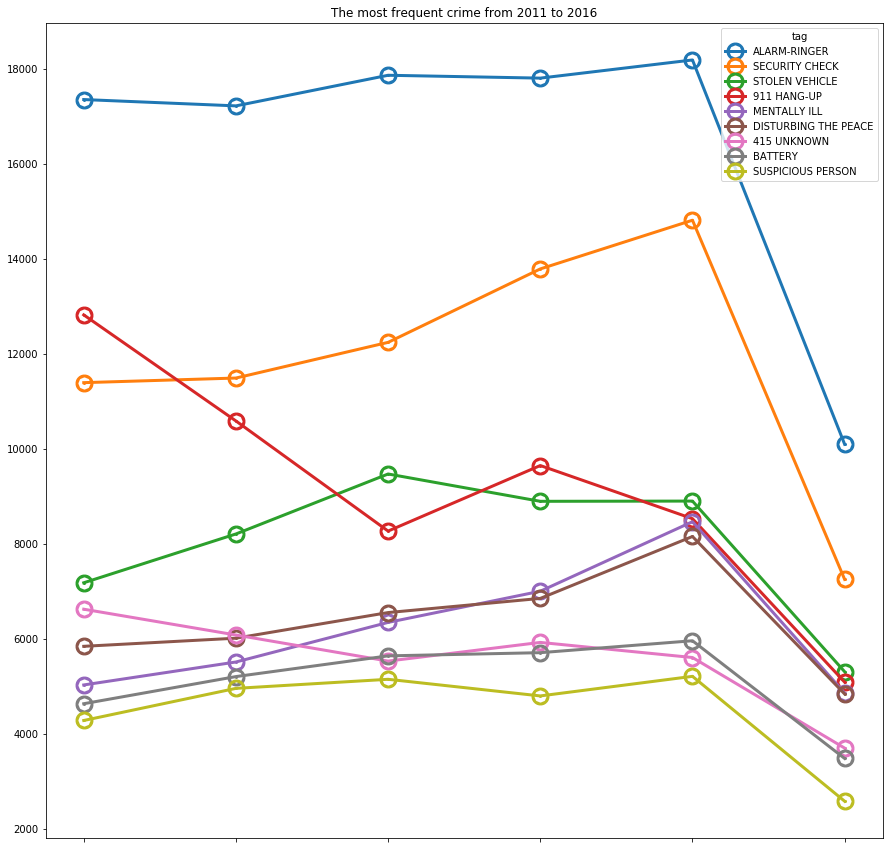
\includegraphics[height=6cm, width=9cm]{1.png}
	\end{center}
	\caption{\hyperref[appendix:plot1]{The most frequent crime in Oakland from 2011 to 2016}}
\end{figure}


\subsection{What crime has the highest occurrence in each location?}


\begin{figure}[H]
	\begin{center}
		%\framebox[4.0in]{$\;$}
		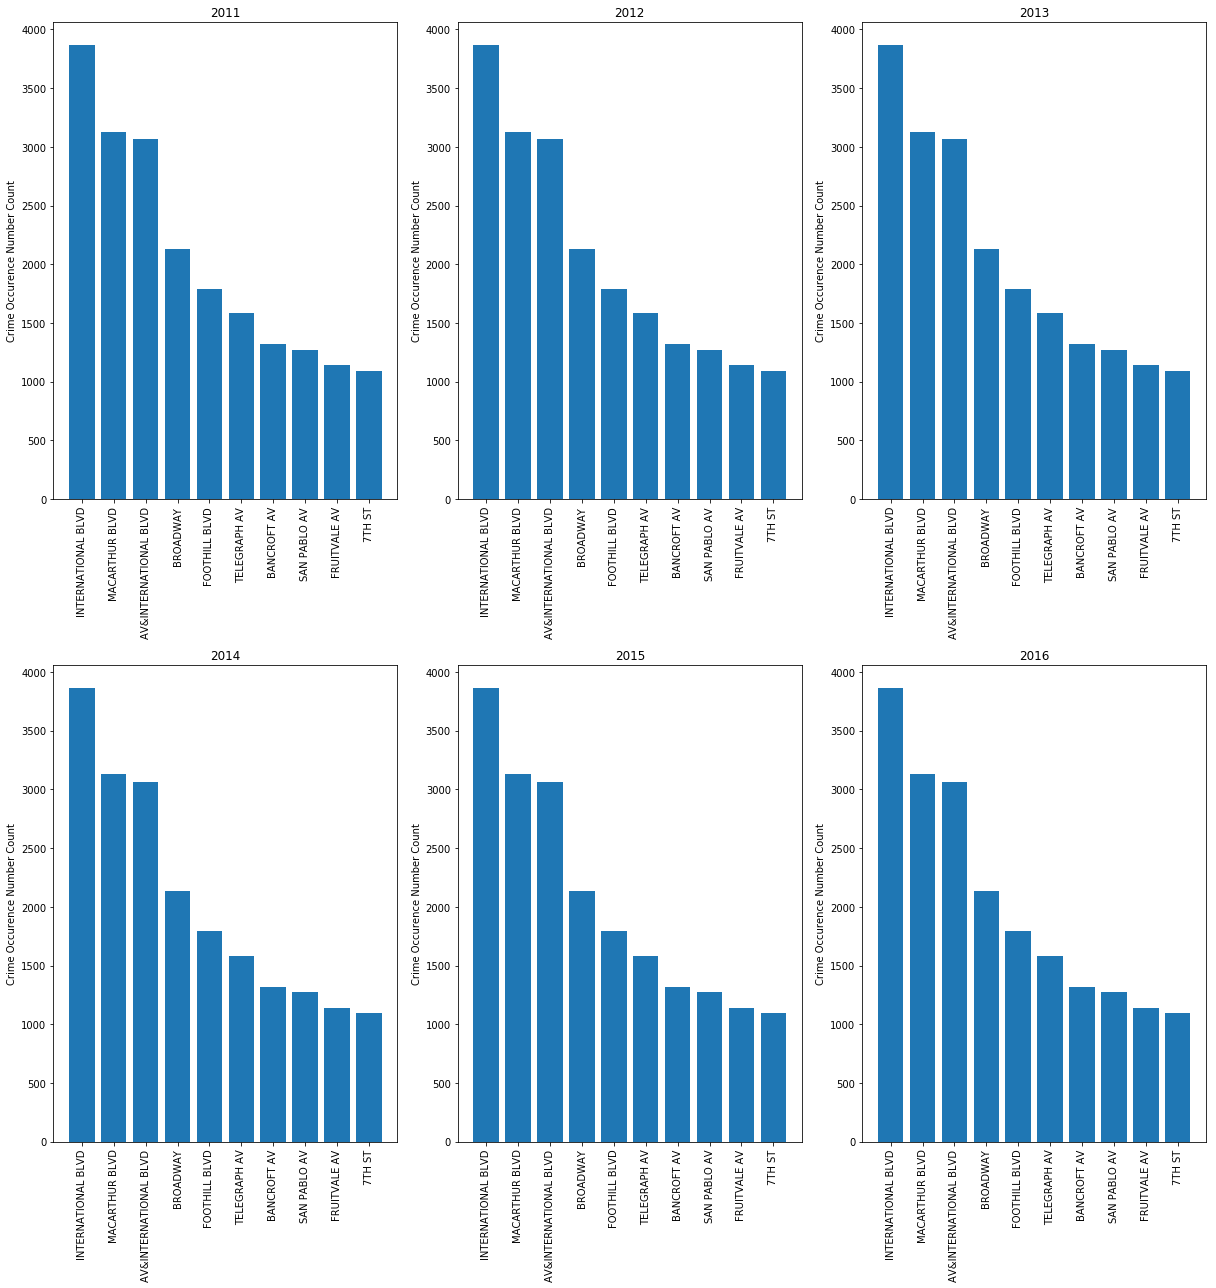
\includegraphics[height=8cm, width=15cm]{2.png}
	\end{center}
	\caption{\hyperref[appendix:plot1]{Locations with the most frequent crime in Oakland from 2011 to 2016}}
\end{figure}

The top locations with the most crime reporting counts across 6 years:

\begin{center}
\begin{tabular}{|l|p{3cm}|p{2.2cm}|r|r|r|r|}
	\toprule
	Year & INTERNATIONAL BLVD &  MACARTHUR BLVD &  BROADWAY &  FOOTHILL BLVD &  TELEGRAPH AV &  7TH ST \\
	\midrule
	2011 &                3866 &            3129 &      2132 &           1791 &          1584 &    1093 \\
	2012 &                3658 &            3335 &      2167 &           1649 &          1623 &    1183 \\
	2013 &                3647 &            3002 &      2036 &           1650 &          1558 &    1246 \\
	2014 &                3713 &            2812 &      1996 &           1774 &          1573 &    1285 \\
	2015 &                3695 &            3105 &      2407 &           1753 &          1507 &    1569 \\
	2016 &                2156 &            1813 &      1476 &           1052 &           875 &    1224 \\
	\bottomrule
\end{tabular}
\end{center}

\begin{figure}[H]
	\begin{center}
		%\framebox[4.0in]{$\;$}
		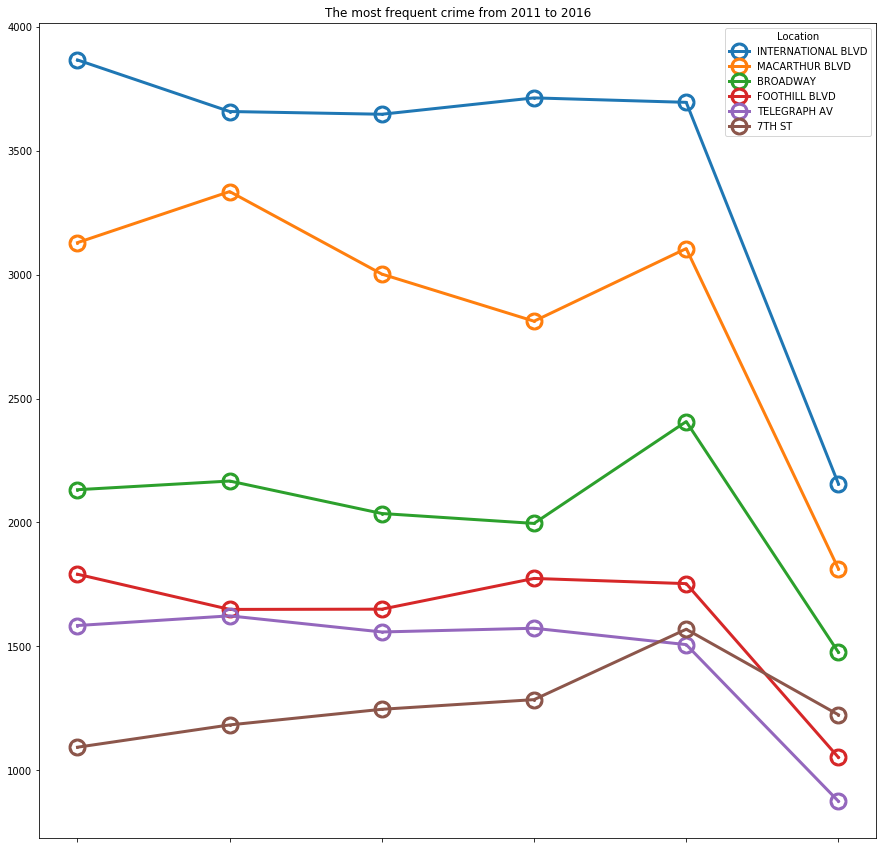
\includegraphics[height=8cm, width=9cm]{3.png}
	\end{center}
	\caption{\hyperref[appendix:plot2]{The location with highest crime rate from 2011 to 2016}}
\end{figure}

Therefore, observing from the graph above, the \textbf{International Blvd} is the place with the highest crime reporting rate.


\subsubsection{What crime has the highest occurrence in International Blvd?}

The top incident types with the highest reporting counts in \textbf{International Blvd} across 6 years:

\begin{center}
\begin{tabular}{|p{1cm}|p{6cm}|p{3cm}|}
	\toprule
	{} &            crime type &  occurrence \\
	\midrule
	0 &          ALARM-RINGER &        1979 \\
	1 &           911 HANG-UP &        1646 \\
	2 &  DISTURBING THE PEACE &        1009 \\
	3 &          MENTALLY ILL &         911 \\
	4 &           415 UNKNOWN &         984 \\
	5 &               BATTERY &         723 \\
	6 &        SECURITY CHECK &        1456 \\
	7 &        STOLEN VEHICLE &         725 \\
	\bottomrule
\end{tabular}
\end{center}


\begin{figure}[H]
	\begin{center}
		%\framebox[4.0in]{$\;$}
		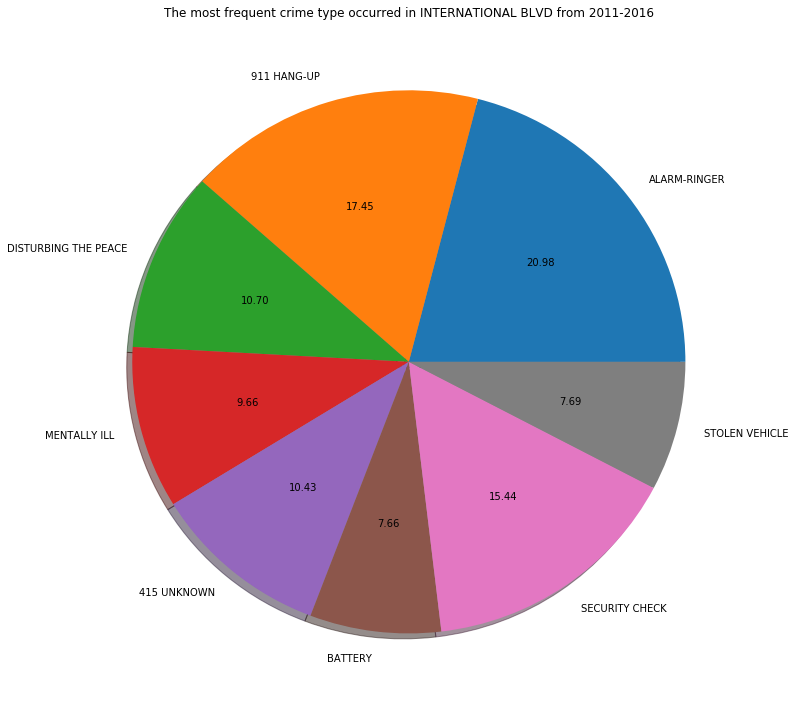
\includegraphics[height=8cm, width=8cm]{4.png}
	\end{center}
	\caption{\hyperref[appendix:plot3]{The most frequent crime type reported in International Blvd from 2011-2016}}
\end{figure}




\subsection{What is the incident solving time for each incident?}


\begin{figure}[H]
	\begin{center}
		%\framebox[4.0in]{$\;$}
		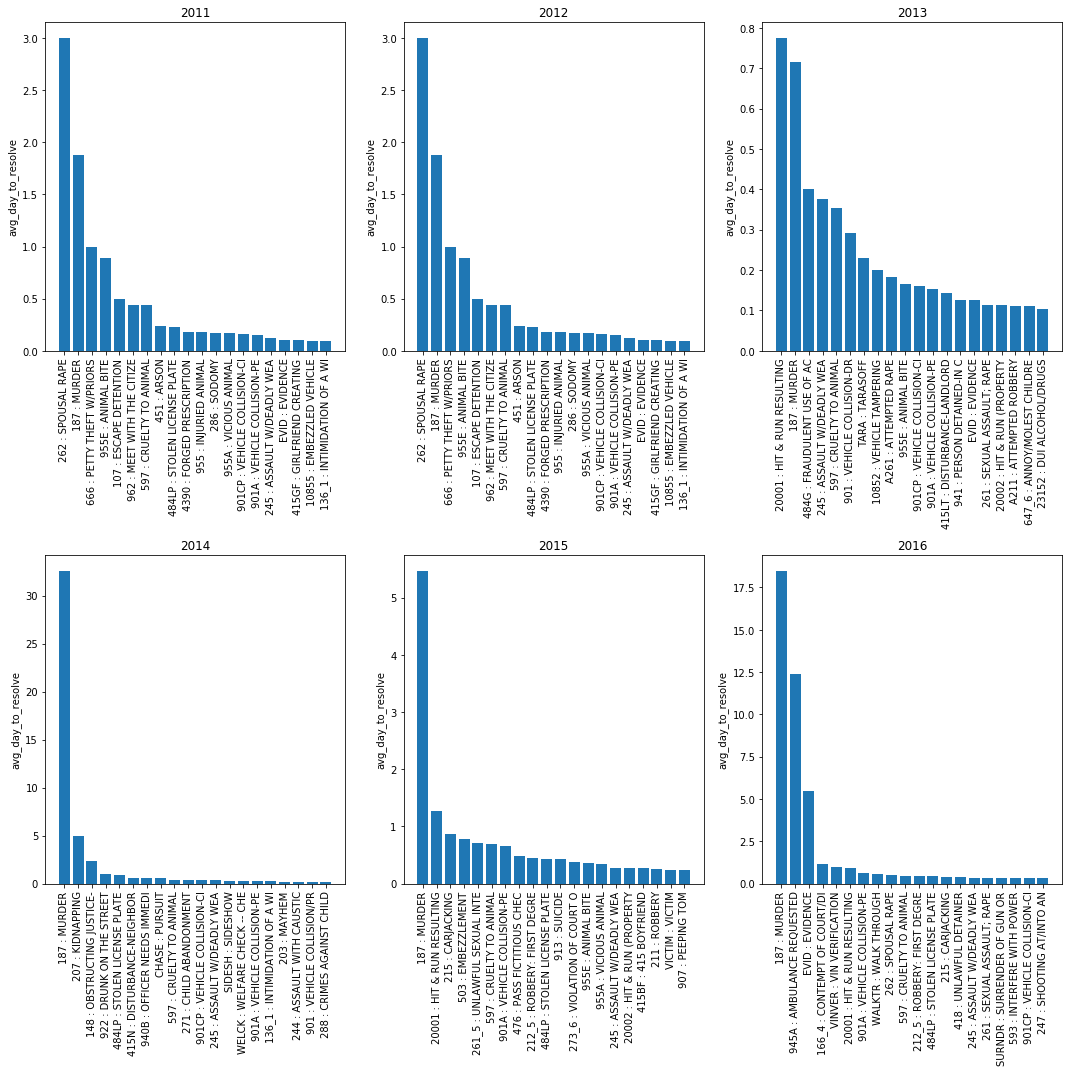
\includegraphics[height=8cm, width=15cm]{5.png}
	\end{center}
	\caption{\hyperref[appendix:plot4]{The average resolving time of crime types in Oakland from 2011-2016}}
\end{figure}


The average resolving days of the top incident types that took the longest days to resolve from 2011 to 2016:

\begin{center}
\begin{tabular}{|l|r|r|r|r|r|}
	\toprule
	 &   MURDER &  ANIMAL BITE &  CRUELTY TO ANIMAL &  VICIOUS ANIMAL &  VEHICLE COLLISION-PE \\
	\midrule
	2011 &   1.8750 &       0.8884 &             0.4347 &          0.1660 &                0.1542 \\
	2012 &   0.7143 &       0.1660 &             0.3531 &          0.0738 &                0.1524 \\
	2013 &  32.5758 &       0.1453 &             0.4140 &          0.1200 &                0.2821 \\
	2014 &   5.4688 &       0.3646 &             0.6883 &          0.3364 &                0.6486 \\
	2015 &  18.4839 &       0.1588 &             0.4433 &          0.1555 &                0.6310 \\
	2016 &   5.4118 &       0.2806 &             0.5074 &          0.1727 &                0.1474 \\
	\bottomrule
\end{tabular}
\end{center}

\begin{figure}[H]
	\begin{center}
		%\framebox[4.0in]{$\;$}
		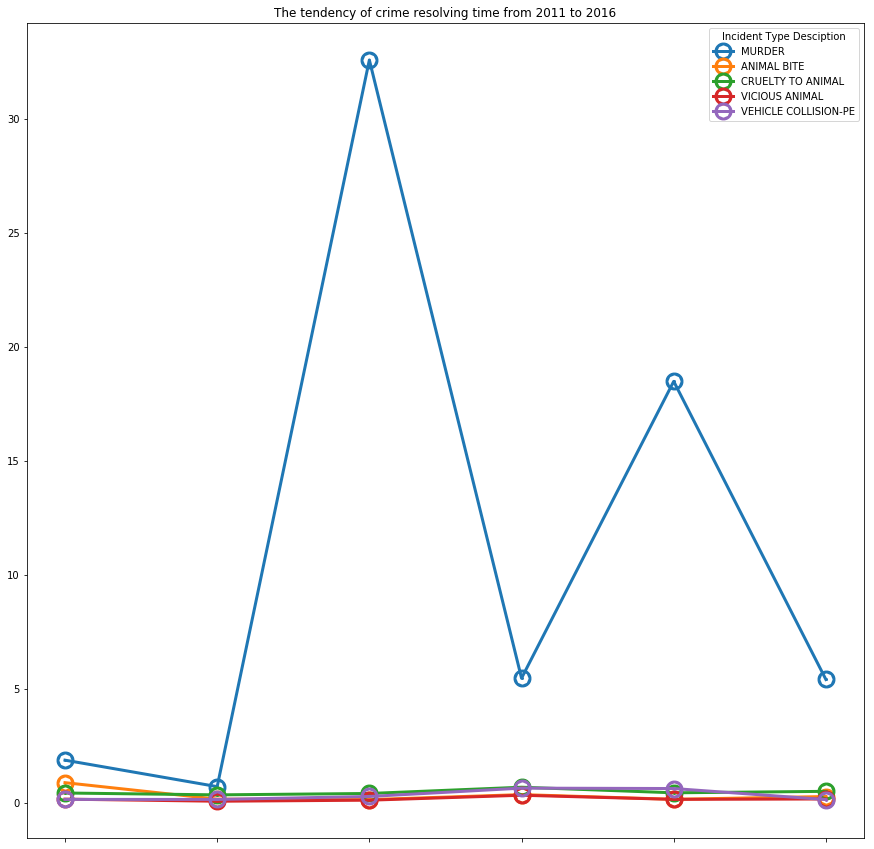
\includegraphics[height=7cm, width=9cm]{6.png}
	\end{center}
	\caption{\hyperref[appendix:plot4]{The time cost trend of top incident types that took the longest resolving time  from 2011 to 2016}}
\end{figure}

\section{Discussion}
In retrospect, we run into a few blocks and encounter several challenges throughout the implementation of the project. For instance:

\begin{itemize}
\item Which database to use?

Since the IST MySQL server has restriction on the size of data uploaded, and our dataset consists of 6 csv files with each containing approximately 200000 rows, thus we use our local MySQL server for the task instead (in fact, MySQL RDS on AWS works as well, but the latency when executing SQL queries slows down the data extracting and processing, thus for the sake of this project, local MySQL server is a better option. Of course in real-life data processing, things would not be as easy, but it's always a good practice to sample pieces of data onto our localhost server and test out the processing and cleaning code before deploying).

\item Which process is the most time-consuming?

Although the data is collected from Kaggle and already quite well-structured and clean, there are many data cleaning tasks that we need to attend to before successfully insert all the tables into MySQL, including formating the time attribute to make sure it is MySQL compatible in order to calculate the time difference (\textbf{Days took to resolve a reported crime = Time when the file closed - Time when the file opened}), and writing regex pattern to extract information that is useful for us. From this process we got some useful experience of data cleaning and preprocessing. It's quite important to know the general layout and format of the data we got before we do any transformation on it,  otherwise the whole dataset could be messed up by the wrong processing code, which step could not be roll-backed. The tip we got from this part of our project is to always sample from the whole dataset to test on our data preprocessing code.

\item Any failed attempts?

Originally we planned to write up some machine learning algorithms, one for classification and one for regression, to apply on the dataset. However, after fully examining the data including the layout, data type of each  attribute, we then decided to turn to exploratory analysis instead. Since what we got is a historical dataset and there are no unknown data ready to be tagged or predict, therefore the point of constructing a linear regression or a tree-based (Decision Tree, Random Forest, etc.) classification is moot. In this case, if we build a classifier, then the use of doing so would be to explore which exact attributes are the more important determinants of crime occurrence frequency, which unfortunately we are not able to finalize due to time management situation. (It contains lots of work. Since basically all attributes in our dataset are categorical, before constructing the classifier, we will need to do \textbf{one-hot} transformation to convert each attribute into binary format  with high dimension. However this transformation would turn the each dataset into a one large sparse table, then the execution time becomes a new problem, but it would be a good direction to go for future endeavor.)

\end{itemize}

\section{Conclusion}

From this project, we have been exposed to many problems that we have never encountered before: this is the very first time that we are doing a data analysis on such a large volume of data, even for the previous projects we have taken for other data science courses, we have never tackled over 10,000 lines of data. Also, the theme we choose for this project is very close to our daily life, in other words, doing the whole project is a lot of fun. Meanwhile, we must integrate data processing with programming techniques, which means there are a lot of syntax and third-party libraries we need to learn.

As for our research results, we found that: 
\begin{itemize}
	\item Starting from 2011, the incident type that costs most days to investigate was \textbf{Murder} until 2016
	\item the \textbf{International Blvd} is the area where most incidents were reported for the past years
	\item Among all incidents, \textbf{Alarm Ringer} is the most frequently reported type in Oakland as well as the International Blvd
\end{itemize}

To sum up, though it is a time-consuming project, we still learned a lot during the process of solving problems, especially the coding and data processing skill. It is a pleasant journey to apply what we have learned from the class to the real-life problem, which not only gives us a better understanding of MySQL dataset, but also propelled us to learn something extremely useful outside of the class.
\[\]


\bibliographystyle{plain}
\bibliography{ref}





\end{document}
